\section{Removal of the highest correct choice}
\label{app:tables}
For each list with two or more correct choices, we sent the list again without the correct choice with the highest probability, and report the correct choice with the second highest probability. If the other choices kept their ratios, its probability after the removal would be its probability in the full list divided by one minus the probability of the removed choice (\emph{Renorm.}).

\begin{table}[!htbp]
\caption{Mean probability of the second correct choice in the full list (\emph{Before}) and after the removal (\emph{After}).}
\label{tab:removal}
\centering
\resizebox{\linewidth}{!}{\begin{tabular}{lrrrrrrrrrrrr}
\toprule
 & \multicolumn{4}{c}{MetaTool} & \multicolumn{4}{c}{HotpotQA} & \multicolumn{4}{c}{ECtHR} \\
\cmidrule(lr){2-5} \cmidrule(lr){6-9} \cmidrule(lr){10-13}
Model & Before & After & Renorm. & After$^*$ & Before & After & Renorm. & After$^*$ & Before & After & Renorm. & After$^*$ \\
\midrule
Jev & 0.11 & 0.71 & 0.77 & 0.72 & 0.17 & 0.66 & 0.80 & 0.67 & 0.19 & 0.71 & 0.72 & 0.71 \\
Liquid d1 & 0.16 & 0.62 & 0.64 & 0.61 & 0.19 & 0.68 & 0.80 & 0.70 & 0.16 & 0.68 & 0.70 & 0.67 \\
GPT-6 Luna Decisions & 0.11 & 0.53 & 0.40 & 0.49 & 0.16 & 0.60 & 0.61 & 0.60 & 0.15 & 0.68 & 0.59 & 0.68 \\
\bottomrule
\end{tabular}
}
\end{table}

\begin{table}[!htbp]
\caption{Mean probability of the second correct choice after renormalisation (\emph{Renorm.}) and after the removal (\emph{After$^*$}), on the examples in which the choices other than the removed one hold 0.1 or more.}
\label{tab:removal-renormalised}
\centering
\resizebox{\linewidth}{!}{\begin{tabular}{lrrrrrr}
\toprule
 & \multicolumn{2}{c}{MetaTool} & \multicolumn{2}{c}{HotpotQA} & \multicolumn{2}{c}{ECtHR} \\
\cmidrule(lr){2-3} \cmidrule(lr){4-5} \cmidrule(lr){6-7}
Model & Renorm. & After$^*$ & Renorm. & After$^*$ & Renorm. & After$^*$ \\
\midrule
Jev & 0.77 & 0.72 & 0.80 & 0.67 & 0.72 & 0.71 \\
Liquid d1 & 0.64 & 0.61 & 0.80 & 0.70 & 0.70 & 0.67 \\
GPT-6 Luna Decisions & 0.40 & 0.49 & 0.61 & 0.60 & 0.59 & 0.68 \\
\bottomrule
\end{tabular}
}
\end{table}
\FloatBarrier

\section{Calibration}
\label{app:calibration}
\begin{table}[!htbp]
\caption{ECE in percentage points of the confidence on lists with one correct choice.}
\label{tab:calibration-one}
\centering
\footnotesize
\begin{tabular}{lrr}
\toprule
 & \multicolumn{2}{c}{One correct choice} \\
\cmidrule(lr){2-3}
 & \multicolumn{1}{c}{MetaTool} & \multicolumn{1}{c}{ECtHR} \\
\cmidrule(lr){2-2} \cmidrule(lr){3-3}
Model & ECE & ECE \\
\midrule
Jev & 8 & 3 \\
Liquid d1 & 9 & 1 \\
GPT-6 Luna Decisions & 14 & 1 \\
\bottomrule
\end{tabular}

\end{table}

\begin{table}[!htbp]
\caption{ECE in percentage points of the probability of yes on the yes/no questions, over all bins (\emph{All bins}) and without the bin from 0 to 0.1 (\emph{From 0.1}).}
\label{tab:calibration}
\centering
\resizebox{\linewidth}{!}{\begin{tabular}{lrrrrrrrrrr}
\toprule
 & \multicolumn{4}{c}{One correct option} & \multicolumn{6}{c}{Several correct options} \\
\cmidrule(lr){2-5} \cmidrule(lr){6-11}
 & \multicolumn{2}{c}{MetaTool} & \multicolumn{2}{c}{ECtHR} & \multicolumn{2}{c}{MetaTool} & \multicolumn{2}{c}{HotpotQA} & \multicolumn{2}{c}{ECtHR} \\
\cmidrule(lr){2-3} \cmidrule(lr){4-5} \cmidrule(lr){6-7} \cmidrule(lr){8-9} \cmidrule(lr){10-11}
Model & Acc. & Conf. & Acc. & Conf. & Acc. & Conf. & Acc. & Conf. & Acc. & Conf. \\
\midrule
Jev & 0.79 & 0.88 & 0.89 & 0.86 & 0.98 & 0.86 & 0.97 & 0.78 & 0.95 & 0.74 \\
Liquid d1 & 0.72 & 0.81 & 0.88 & 0.87 & 0.91 & 0.74 & 0.96 & 0.76 & 0.96 & 0.74 \\
GPT-6 Luna Decisions & 0.73 & 0.87 & 0.90 & 0.89 & 0.82 & 0.74 & 0.95 & 0.75 & 0.96 & 0.74 \\
\bottomrule
\end{tabular}
}
\end{table}

\begin{figure*}[t]
\centering
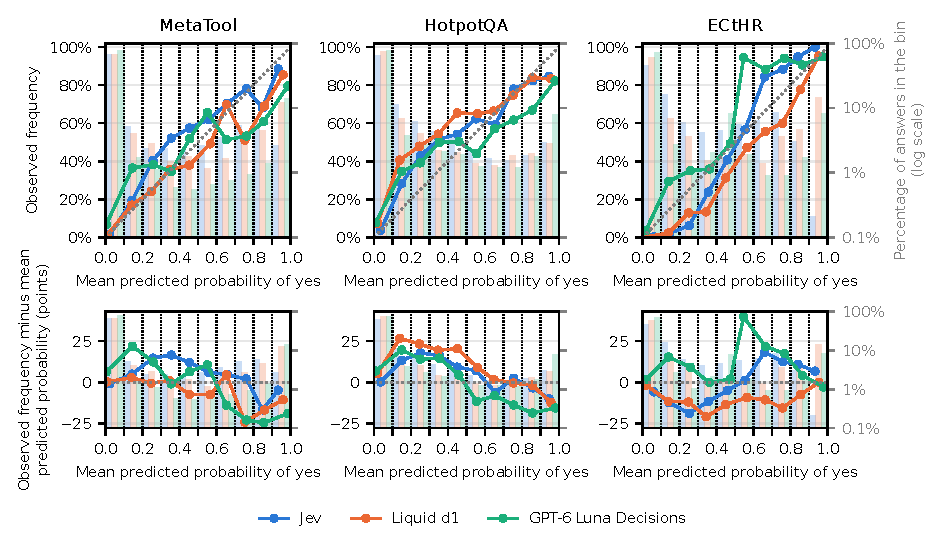
\includegraphics[width=\linewidth]{figures/reliability}
\caption{Reliability diagram of the yes/no questions on examples with two or more correct choices, in bins of width 0.1. Each point is at the mean probability of yes of its bin. Top: the observed frequency of correct choices. Bottom: the observed frequency minus the mean probability, in percentage points. The bars give the share of the answers in each bin, on a log scale.}
\label{fig:reliability}
\end{figure*}
